\documentclass[12pt]{article}
%------------------------------Packages généraux------------------------------

\usepackage[french]{babel}
\usepackage[T1]{fontenc}
\usepackage{ae}
\usepackage[utf8]{inputenc}
\usepackage{lmodern}
\usepackage[a4paper,left=2.5cm,right=2.5cm,top=2cm,bottom=3cm]{geometry}
%------------------------------Mathématiques------------------------------

\usepackage{amsmath}
\usepackage{amssymb}
\usepackage{amsthm}
\usepackage{amsfonts}
\usepackage{eucal}
\usepackage{array}


%------------------------------Graphics------------------------------

\usepackage{caption}
\usepackage{subcaption}
\usepackage{graphicx}
\usepackage{fancyhdr}
\usepackage{fancybox}
\usepackage{color}
\usepackage{epstopdf}
\usepackage{float}
\usepackage{diagbox}
\usepackage{framed}

%------------------------------Syntaxe------------------------------

\usepackage{listings}
\usepackage{color} %red, green, blue, yellow, cyan, magenta, black, white
\definecolor{mygreen}{RGB}{28,172,0} % color values Red, Green, Blue
\definecolor{mylilas}{RGB}{170,55,241}
\lstloadlanguages{Matlab}

\def\refmark#1{\hbox{$^{\ref{#1}}$}}
\DeclareSymbolFont{cmmathcal}{OMS}{cmsy}{m}{n} %Mathcal correcte
\DeclareSymbolFontAlphabet{\mathcal}{cmmathcal}

\setlength{\parskip}{1ex plus 0.5ex minus 0.2ex}
\newcommand{\hsp}{\hspace{20pt}}
\newcommand{\HRule}{\rule{\linewidth}{0.5mm}}




\begin{document} 


\begin{titlepage}


  \begin{sffamily}
  \begin{center}

   
    \textsc{\Large Université de Liège}\\[0.8cm]
    
    \begin{figure}[h!]
		\begin{center}
		\includegraphics[scale=1.2]{logoULG}\\[1cm]
		\end{center}
	\end{figure}
	

    \textsc{\Large Eléments de processus stochastiques}\\[1.1cm]

    
    \HRule \\[0.4cm]
    { \LARGE \bfseries Méthodes de Monte Carlo par chaines de Markov - application à la cryptanalyse \\[0.4cm] }

    \HRule \\[0.5cm]
    
    \textsc{3\up{ème} bachelier en ingénieur civil} \\[2.5cm]

   \begin{minipage}{0.4\textwidth}
      \begin{flushleft} \large
        \emph{Auteurs:}\\
        Tom \textsc{Crasset} \\
        Antoine \textsc{Louis}  \\
        Romain \textsc{Vaneukem} \\
      \end{flushleft}
    \end{minipage}
    \begin{minipage}{0.4\textwidth}
      \begin{flushright} \large
        \emph{Professeur :}\\
        V. \textsc{Denoël}\\[0.5cm]
      
        \emph{Assistant:}\\
        L. \textsc{Duchesne}\\
        
      \end{flushright}
    \end{minipage}

    \vfill
    
    {\large Année académique 2017-2018}

  \end{center}
  \end{sffamily}
\end{titlepage}


\section{Chaînes de Markov pour la modélisation du langage et MCMC}
\subsection{Chaîne de Markov pour la modélisation du langage}

\subsubsection*{Question 1}
La méthode de vraisemblance a pour but de trouver la valeur du paramètre $\theta$ qui maximise la probabilité de trouver l'échantillon $ D_n$ qui ici est la séquence donnée par \texttt{seq1}. D'un point de vue théorique nous avons, $$  \hat{\theta}_{MV} = arg(max_{\substack{\theta}} \mathcal{L}(\chi_i ,\theta))$$ avec $$ \mathcal{L}(\chi_i,\theta) = P(D_n \mid \theta) = P((\chi_1, ..., \chi_n) = (x_1, ..., x_n)) $$
les événements étant indépendant,
$$ \mathcal{L}(\chi_i,\theta) = P((\chi_1 = x_1), ..., (\chi_2 = x_n)) = \prod_i P(\chi_i = x_i) $$
Pour trouver la matrice de transition par cette méthode, nous nous basons sur la séquence fournie. Prenons l'exemple de l'élément $\textbf{Q}(2,3)$ qui représente la probabilité de passer de la lettre 'b' à la lettre 'c'. Nous cherchons le nombre total des séquences 'bc' et divisons ce total par le nombre de 'b', ceci nous donnes bien la probabilité recherchée. Cette même méthode peut être appliquée pour la distribution initiale $\pi_0$. Ici, la fréquence d'une lettre est directement divisée par le nombre de lettres et on obtiens ainsi la distribution recherchée.
\paragraph{}Voici les résultats numériques,
$$ \textbf{Q}=\begin{bmatrix}
0 & 0.0857 & 0.1 & 0.8143
\\1 & 0 &0 &0
\\0.6744 &0 &0 &0.3256
\\0.3662 & 0.1268 &0.507 &0
\end{bmatrix}$$
% Partie qui peut être tronquée si on dépasse la longueur de page
On remarquera de cette matrice quelques éléments intéressants. La diagonale est nulle, c'est-à-dire que la probabilité qu'une séquence aie deux fois la même lettre qui se suit est nulle. Chaque élément nulle de cette matrice montre un événement impossible, il est donc impossible que la lettre "b" précèdent la lettre "c". Il y a une probabilité certaine que la "b" sera suivie par la lettre "a" car $ \textbf{Q}(2,1) = 1$.

Pour la distribution de probabilité initiale nous avons,
$$\pi_0 = \left(\begin{array}{c}0.355\\ 0.075\\ 0.215\\ 0.355 \end{array}\right)$$
Nous pouvons voir à la Figure \ref{etatChaineMarkov}, le diagramme d'états de la chaîne de Markov.
\begin{figure}[!h]
\begin{framed}
      \centering
      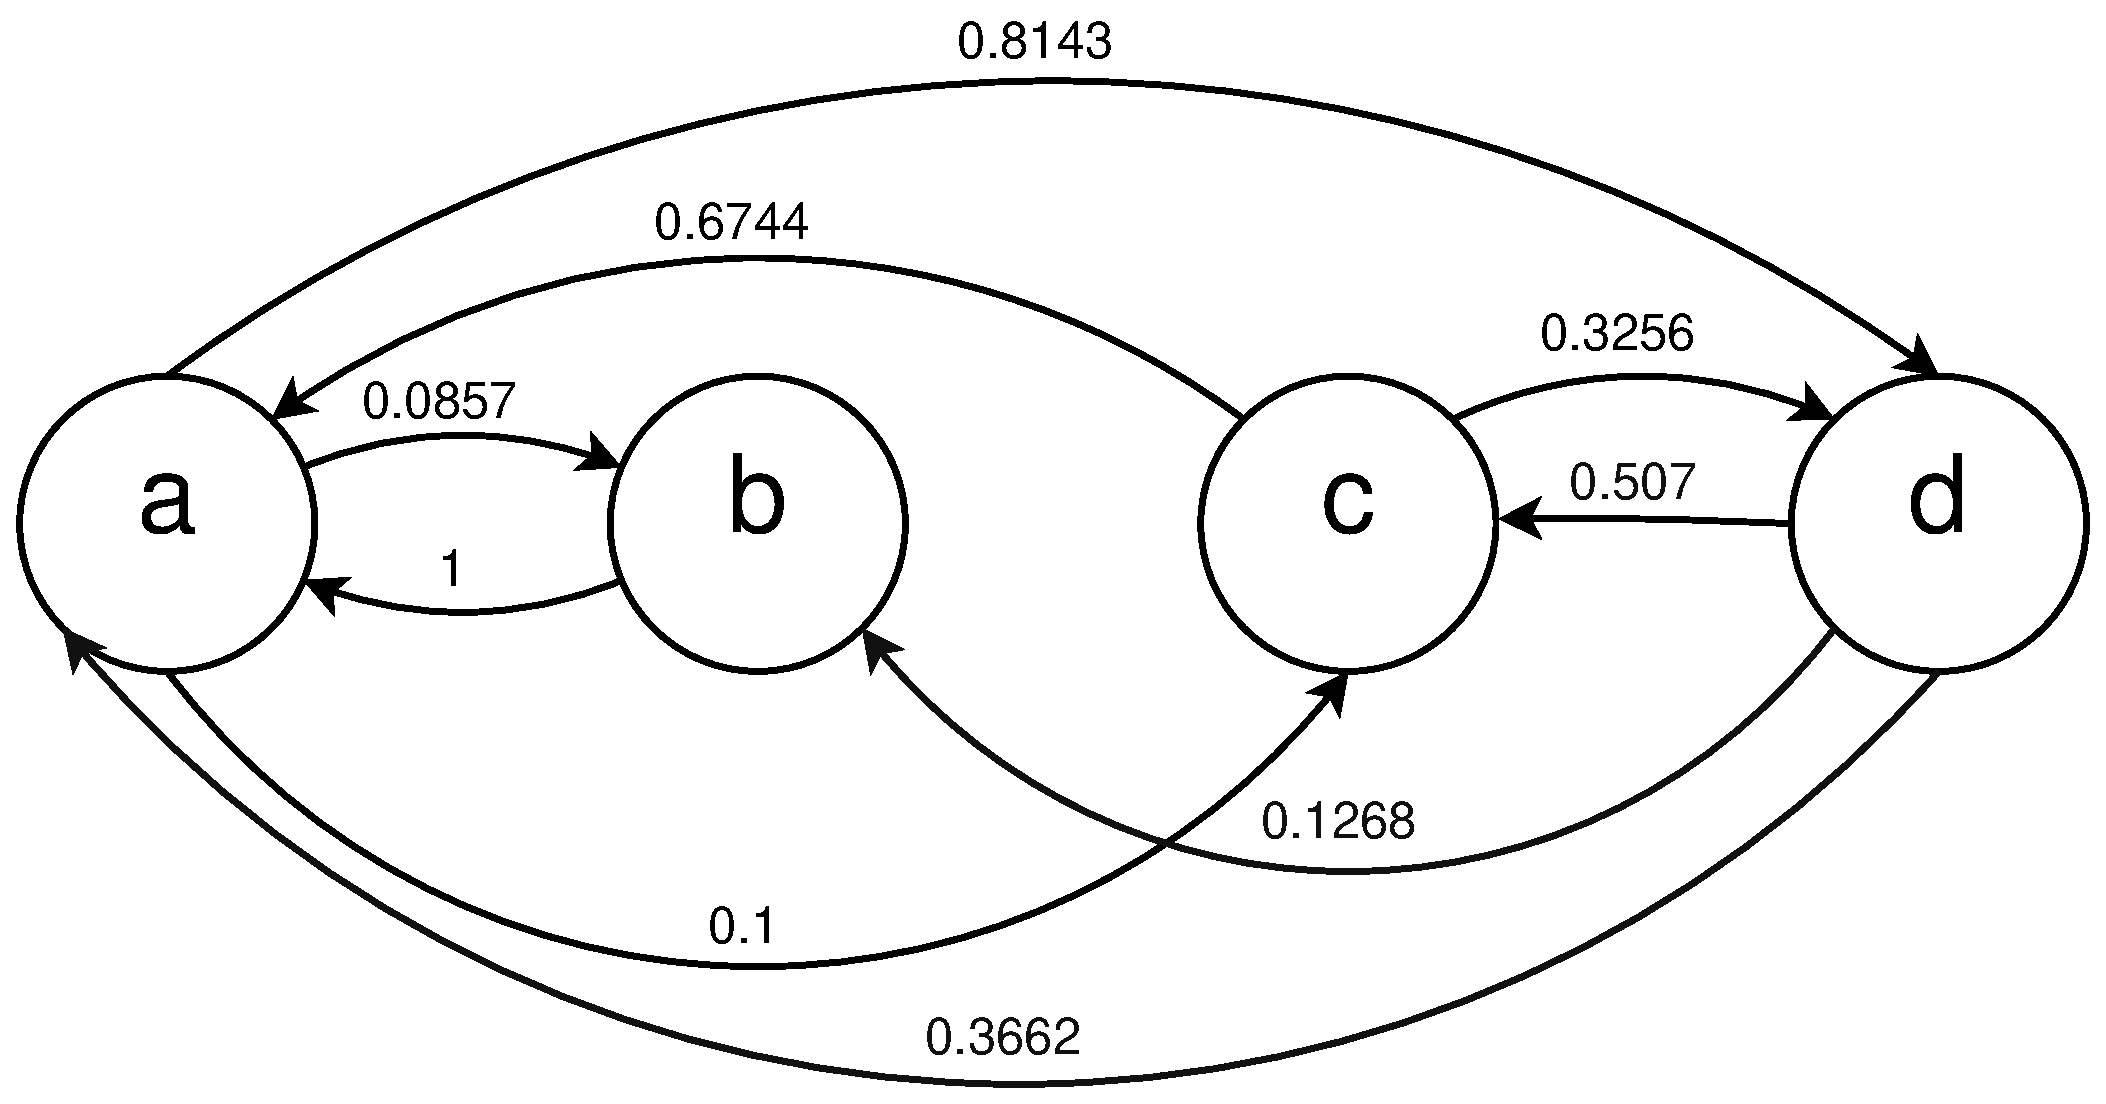
\includegraphics[scale=0.23]{DiagrammeetatdeChaine.eps}
       \caption{Diagramme d'états de la chaîne de Markov}
       \label{etatChaineMarkov}
  \end{framed}
  \end{figure}
  
\subsubsection*{Question 2}
Maintenant que la matrice de transition a pu être calculée, il nous est possible de réaliser quelques opérations. Dans un premier temps, nous supposons que la première lettre est choisie aléatoirement, cela correspond à une distribution de probabilité initiale uniforme: $\pi_0 = \begin{bmatrix}
0.25 & 0.25 & 0.25 & 0.25
\end{bmatrix}$. Pour obtenir les probabilité successive $P(X_t = i)$, il suffit de multiplier chaque densité par la matrice de transition. C'est-à-dire effectuer,
$$ \pi_{n+1} = \pi_n \times \textbf{Q}\ $$
pour $n$ allant de $0$ à $t-1$. Graphiquement nous obtenons le résultat suivant de la Figure \ref{ProbgraphBegin_random}.

 \begin{figure}[!h]
      \centering
      \includegraphics[scale=0.5]{uniformDist.eps}
       \caption{Représentation graphique de $P(X_t = i)$ avec i = 'a','b','c','d' partant d'une lettre aléatoire}
       \label{ProbgraphBegin_random}

  \end{figure}
 
Il nous est demandé aussi de représenter cette probabilité $P(X_t = i)$  en commençant par la lettre 'c'. La différence ici est la distribution de probabilité initiale: 
$\pi_0 = \begin{bmatrix}
0 & 0 & 1 & 0
\end{bmatrix}$
, ce graphique peut être observé à la Figure \ref{ProbgraphBegin_c}.


 \begin{figure}[!h]
      \centering
      \includegraphics[scale=0.5]{startOnC.eps}
       \caption{Représentation graphique de $P(X_t = i)$ avec i = 'a','b','c','d' partant de la lettre 'c'}
       \label{ProbgraphBegin_c}

  \end{figure} 
  
  
 % /!\      !!!!!!!!Ne pas OUBLIER!!!!!    /!\
 %La discussion par rapport a la théorie est à faire
 %
 %!!!!!!!!!!!!!!!!!!!!!!!!!!!!!!!!!!!!!!!!!!!!!!!!!!!!!!!!!!!!
Par rapport à la théorie, la matrice $\textbf{Q}$ permet de passer d'un état à un autre. C'est-à-dire la probabilité conditionnelle, $$Q_n(i,j) = P(\chi_{n+1} = j|\chi_n = i_n)$$
A partir de la distribution initial et de la matrice de transition on peut caractériser entièrement la fonction de probabilité conjointe de la chaîne de Markov. En effet, par définition,
$$P(\chi_1 = i_1,X_0 = i_0) = P(X_1 = i_1|X_0 = i_0)P(\chi_0 = i_0)$$
On peut aussi s’intéresser à la fonction de probabilité conjointe entre les trois premières lettres.
$$P(\chi_2 = i_2,\chi_1 = i_1,\chi_0 = i_0) = P(\chi_2 = i_2|\chi_1 = i_1,\chi_0 = i_0)P(\chi_1 = i_1,\chi_0 = i_0)$$
Par définition d'une chaîne de Markov, un événement $n$ vers un événement $n+1$ ne dépend pas de l'historique. Alors,
$$P(\chi_2 = i_2,\chi_1 = i_1,\chi_0 = i_0) = P(\chi_2 = i_2|\chi_1 = i_1,)Q(i_1,i_0)\pi_0 = Q(i_1,i_2)Q(i_0,i_1)\pi_0$$
Et par récurrence,
$$P(\chi_n = i_n, ..., \chi_0 = i_0) = \pi_0 \prod_{k=1}^n Q(i_{k-1},i_k)$$
On peut observé que dans les évolutions représentée ici, les valeurs tend, lorsque $t$ deviens de plus en plus grand vers une distribution déterministe. Lorsque $t$ tends vers l’infini nous obtenons la distribution de probabilité stationnaire celle-ci va être étudiée plus en détail dans la question suivante.
 %!!!!!!!!!!!DISCUSSION THEORIQUE NON COMPLET!!!!!!!!!!!!!!!!!!
\subsubsection*{Question 3}
Nous allons trouver la distribution de probabilité stationnaire par application direct de sa définition. C'est-à-dire,
$$ [\pi_{\infty}]_j =  \lim_{t \rightarrow \infty} P(\chi_t = j)$$
En pratique, il est question de trouver un $t$ suffisamment grand pour quitter la période transitoire. Nous pouvons le vérifier graphiquement comme représenter à la Figure \ref{stationaryperiod}.

% Le graphique Ci dessous n'est pas obligatoire si on excède la taille de projet (!Texte a modifier, si supprimer)

 \begin{figure}[!h]
      \centering
      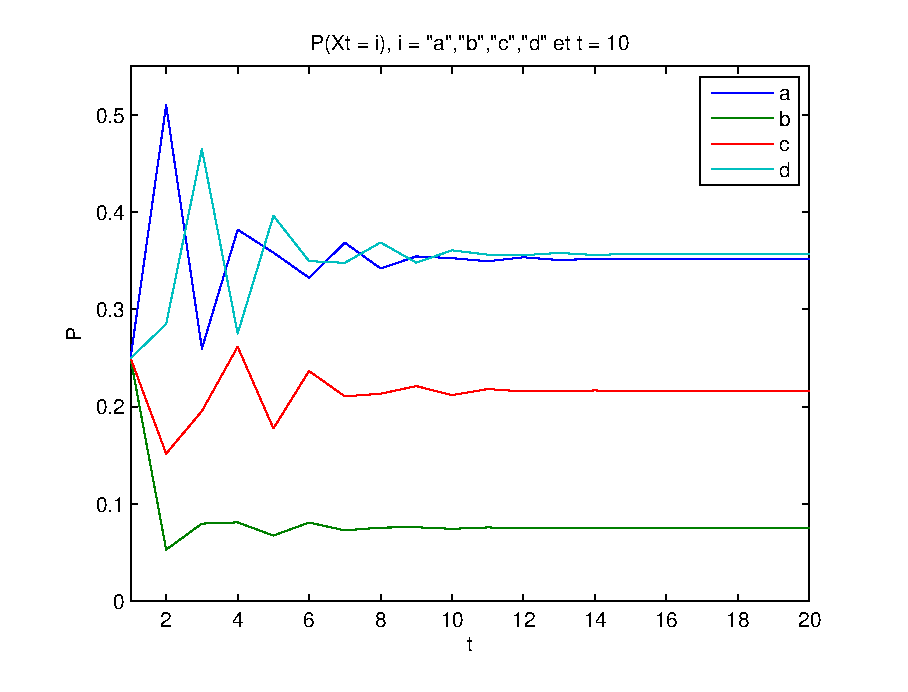
\includegraphics[scale=0.5]{stationnarity.eps}
       \caption{Représentation graphique de la période stationnaire}
       \label{stationaryperiod}
  \end{figure}
On peut observer qu'un $t$ allant jusqu’à 20 est suffisant pour atteindre la stationnarité avec une distribution initiale uniforme. On obtiens,
$$ \pi_{\infty} =   \begin{bmatrix}
0.3517 & 0.0754 & 0.2161 & 0.3568
\end{bmatrix}$$
%0.3517    0.0754    0.2161    0.3568
\subsubsection*{Question 4}
Ils nous est demandé ici de générer une chaîne de Markov en démarrant d'une lettre choisie selon la distribution stationnaire. Chaque lettre est ensuite choisie aléatoirement selon la matrice de transition. Par exemple, si nous nous trouvons à la lettre 'a', la lettre suivante est choisie selon les probabilités: $P(\chi = a) = 0, P(\chi = b) = 0.0857, P(\chi = c) = 0.1, P(\chi = d) = 0.8143$.

Voici un exemple de réalisation pour une longueur de chaîne de 20: '\texttt{dcacadcadcacadbabadadcadadcada}'

On peut comparer la distribution de probabilité de cette chaîne générée avec la distribution stationnaire, en regardant la fréquence de chaque lettre et la diviser par la longueur de chaîne totale.

Les résultats en fonction de la longueur de chaîne sont disponibles à la Table \ref{chainProbaDistrib}. 
\begin{table}[!h]
\centering
\label{my-label}
\begin{tabular}{|l||l|l|l|l|l|l|l||l|}
\hline
 $T$& $P(\chi = a)$&$ P(\chi = b)$  & $ P(\chi = c)$ & $ P(\chi = d)$ \\ \hline \hline
20 &0.3&0.05&0.2&0.45\\ \hline
50 &0.34&0.08&0.22&0.36  \\ \hline
100 &0.37&0.11&0.18&0.34  \\ \hline
170 &0.3706&0.1&0.1765&0.3529  \\ \hline
230&0.3435&0.0609&0.2478&0.3478  \\ \hline
600 &0.3517&0.0733&0.2217&0.3533  \\ \hline \hline
$\pi_{\infty}$&0.3517&0.0754&0.2161&0.3568  \\ \hline
\end{tabular}
\caption{Distribution de probabilités des chaînes générées, où $T$ est la longueur de chaîne}
\label{chainProbaDistrib}
\end{table}
La distribution de probabilité stationnaire a été rappelé pour permettre une comparaison plus aisée. On peut observer que les valeurs de la distribution de probabilités de la chaîne générée se rapproche de plus en plus de la distribution stationnaire de la chaîne qui nous a été donné. La différence est d'autant plus petite que $T$ est élevée et on voit qu'a partir de 600 lettres les valeurs sont relativement proches.
\subsubsection*{Question 5}
Lors de cette expérience, nous sommes parti d'une séquence donnée et étudier sa répartition pour ensuite pourvoir simulé une chaîne similaire.% A reformuler peut-être 
La méthode de vraisemblance nous a parmi de caractériser la séquence donnée et définir sa représentation probabiliste. A partir de cette représentation, il nous a été possible de générée une séquence similaire.
% Cette figure n'est pas totalement obligatoire si on est out de place 
\begin{figure}[!h]
\begin{framed}
      \centering
      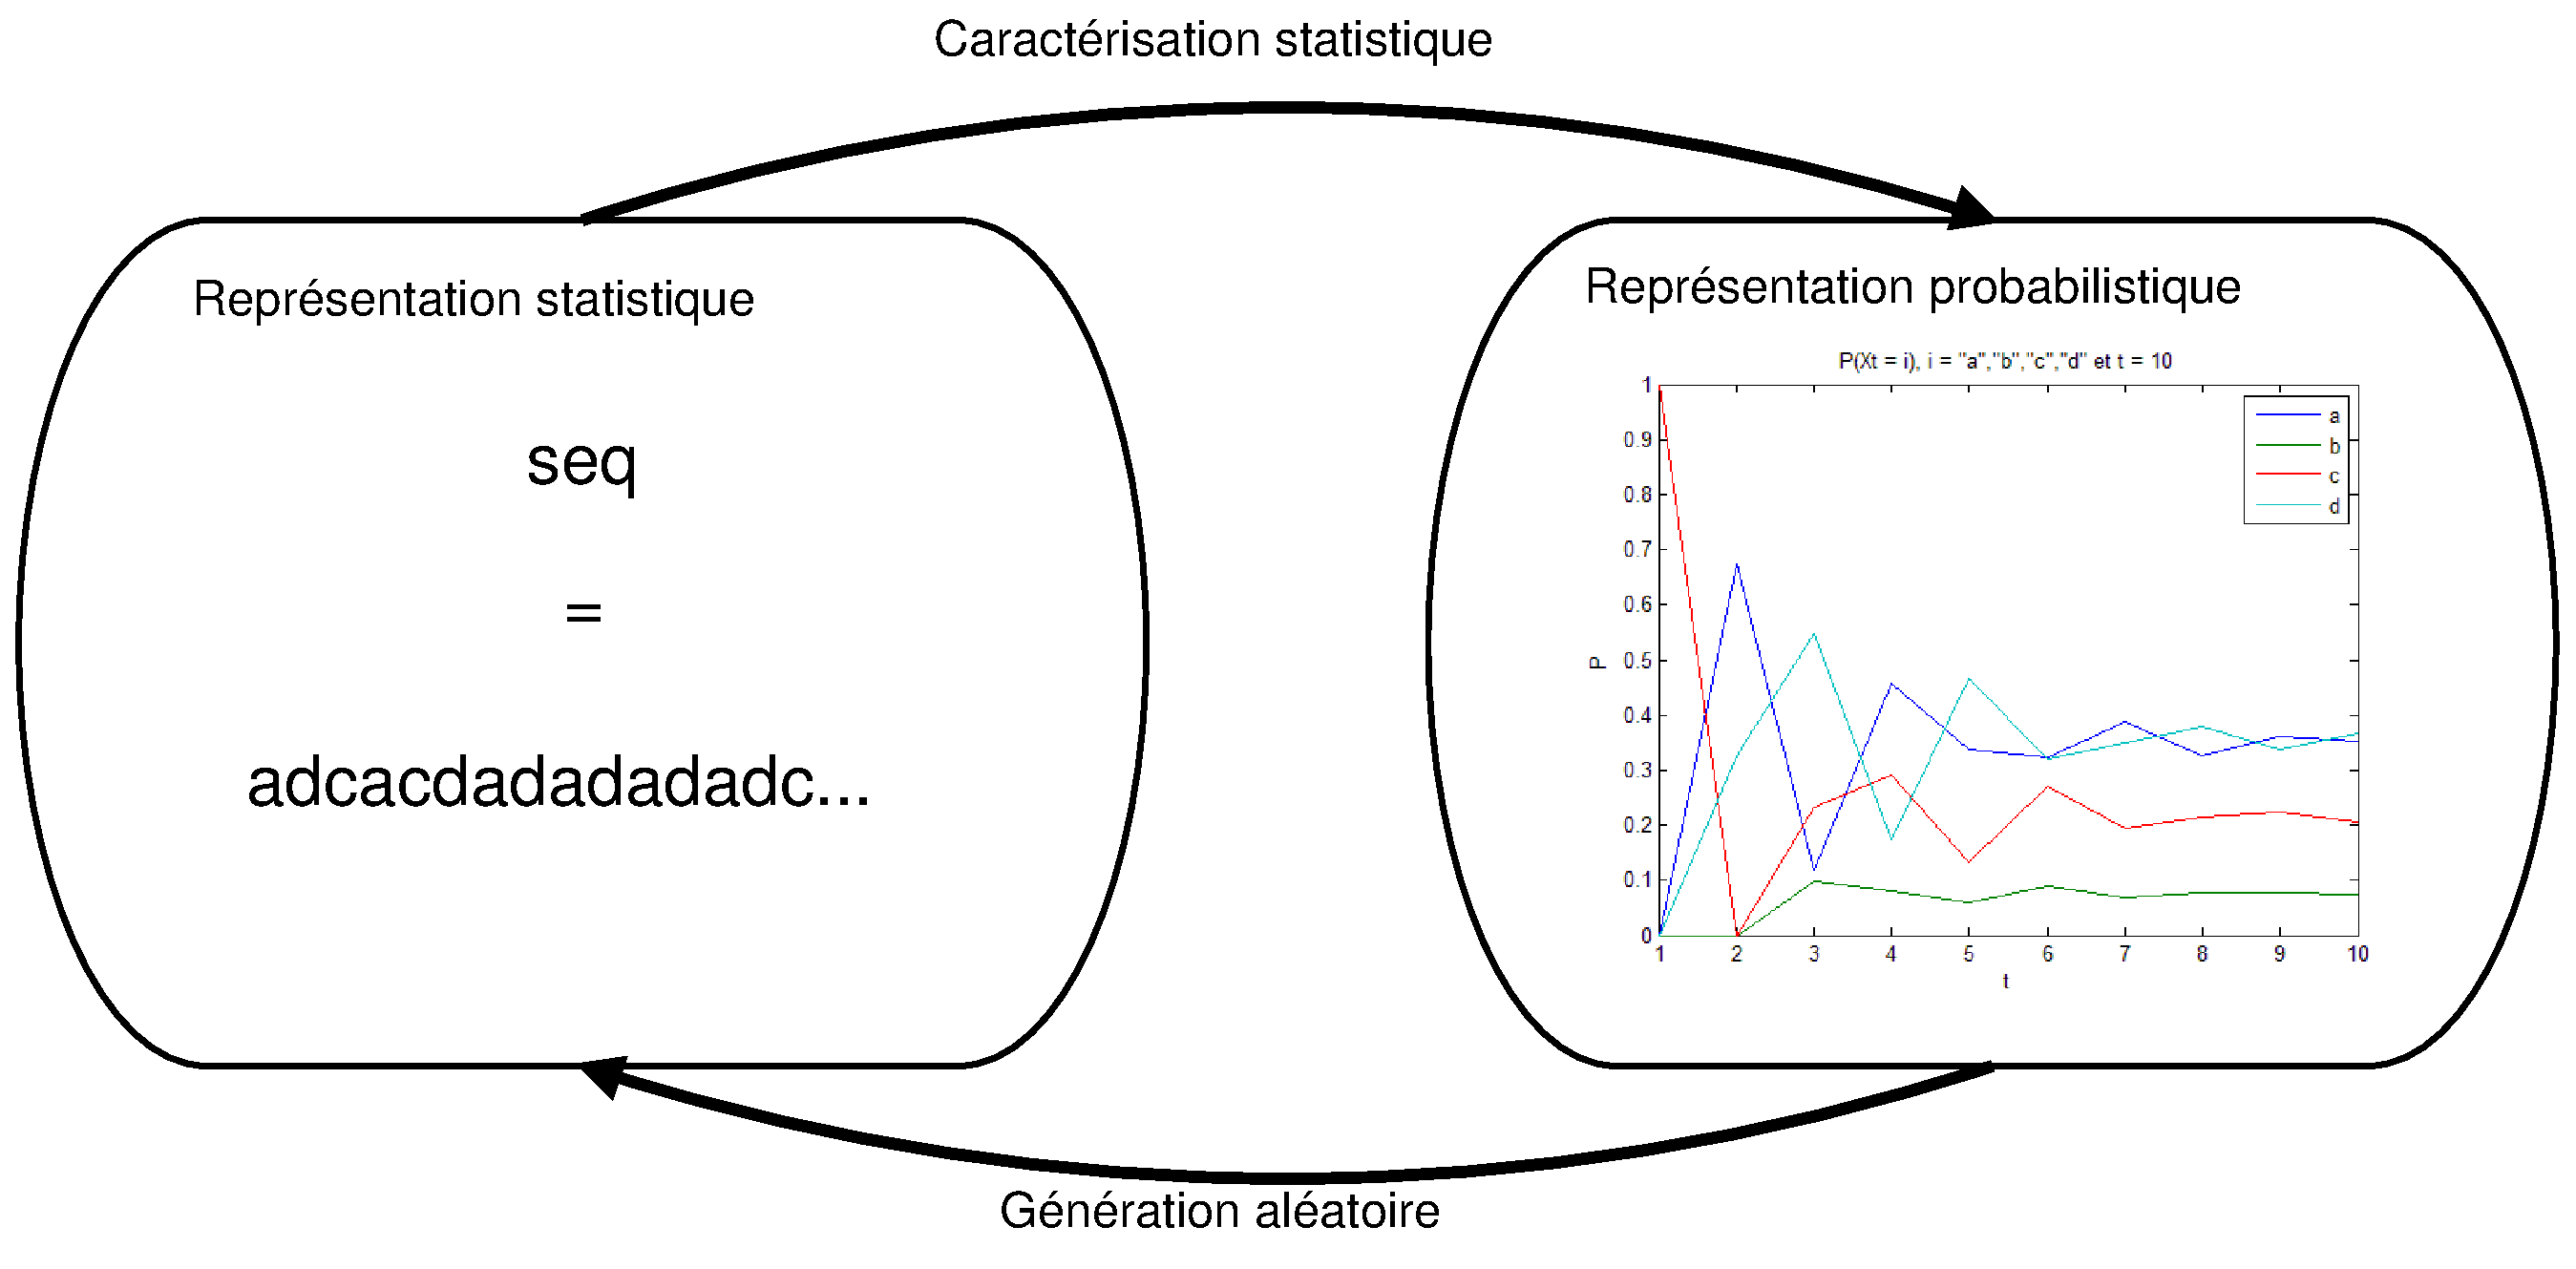
\includegraphics[scale=0.18]{DiaTheo.eps}
       \caption{Deux représentations équivalentes du processus aléatoire}
       \label{ProcessDia}
  \end{framed}
  \end{figure}
Nous pouvons voir à la Figure \ref{ProcessDia}, la démarche suivi lors des questions précédentes .
%!!!!!!!!!!!!!!!!!!!!!A continuer !!!!!!!!!!!!!!!!!!!!!

\subsection{Algorithme MCMC}
\subsubsection*{Question 1}
\paragraph{Stationnarité}
Une distribution de probabilités est dite invariante ou stationnaire lorsque $$\pi_s = \pi_sQ$$

%%%%%%% Pas sur que c'est ce qu'on cherche @Antoine%%%%%%
Une propriété importante d'une distribution stationnaire est que, si la chaine de
Markov est initialisée selon cette distribution, ou s'y retrouve pour une raison ou
pour une autre a un instant k, alors elle y restera pour tous les instants suivants.
En effet, puisque $$\pi_n = \pi_kQ^{n-k} = \pi_kQ...Q = \pi_k$$.
%%%%%%%%%%%%%%%%%%%%%%%%%%%

\paragraph{Equation de balance détaillé}

Une distribution $\pi$ de matrice de transition Q satisfait les équations de balance détaillée si,

\begin{equation}
\pi(i)Q_{ij} = \pi(j)Q_{ji} \qquad ,\forall i,j \in \{1,..,N\}
\end{equation}

Une propriété de cette équation est que toute distribution qui satisfait cette définition est une distribution stationnaire. \\

\underline{Démonstration:}

\begin{equation}
\begin{split}
\pi(j) \stackrel{?}{=} \sum_i{\pi(i)Q_{ij}} & = \sum_i{\pi(j)Q_{ji}} \\
& = \pi(j) \sum_i{Q_{ji}} \\
& = \pi(j) \qquad ,\forall i,j \in \{1,..,N\}
\end{split}
\label{eq2}
\end{equation}

Un exemple heuristique de cette équation de balance détaillée est celui d'un échange de monnaie entre deux (ou plusieurs) personnes.

Si on considère un pas de temps unique de $n$ à $n+1$ pendant lequel chaque personne $i$ a initialement $\pi_i$ euros et paye à chaque personne $j$ une fraction $Q_{ij}$ de celle-ci. La condition d'équilibre détaillée stipule qu'à chaque paiement, l'autre personne paie exactement le même montant d'argent ($\pi_jQ_{ji})$.

Le montant total d'argent que la personne $j$ reçoit (y compris de lui-même) pendant le pas de temps est égal à la somme d'argent qu'il paye aux autres, ce qui équivaut à tout l'argent qu'il avait initialement parce qu'on fait l'hypothèse que tout l'argent est dépensé. ($Q_{ji}$ somme à 1 sur $i$). 
L'argent qui n'est pas vraiment utilisé est simplement considéré comme étant payé de la personne $j$ à lui-même (c'est-à-dire que $Q_{jj}$ n'est pas nécessairement zéro).

%%%%%IL FAUT ENCORE PARLER DE L'UNICITE%%%%%%%









\end{document}
